\documentclass{beamer}
%  Use something like this Perl command to substitute across all files:
% $ perl -p -i -e 's/\\subfolder\//\\dayonesegone\//g' *.tex

% Use jpg graphics in figure environments and pdflatex to compile!!!
\usepackage{graphicx,color,amsmath,amssymb,amsfonts,amsbsy,amsthm}
\usepackage{verbatim}
\usepackage{subcaption}
\usepackage{url} 

\usetheme{Warsaw}
\setbeamertemplate{footline}{}

\newcommand{\includes}{../include}
\newcommand{\graphics}{../graphics}
%\newcommand{\includes}{/home/1104070/latex_include}

\newcommand{\dayonesegtwo}{.}
% Node the following tag will orient things right using dvi2pdf.
% Process with LaTeX first, then dvi2pConstant Velocity Motiondf.
\special{landscape}
% Fuzz -----------------------------------------------------------
\hfuzz5pt % Don't bother to report overfull boxes < 5pt
% MATH -----------------------------------------------------------
\input{\includes/kalman_cmdmaster.tex}
% THEOREM ENV. ---------------------------------------------------
\newtheorem{thm}{Theorem.}
\newtheorem{cor}[thm]{Corollary.}
\newtheorem{con}[thm]{Conjecture.}
\newtheorem{lem}[thm]{Lemma.}
\newtheorem{prop}[thm]{Proposition.}
\newtheorem{defn}[thm]{Definition.}
\renewcommand{\thethm}{}  % unnumbered
%\pagestyle{plain}
%%% --------------------------------------------------------------
\newcounter{exercisecounter}

\begin{document}
\title{
\vfill \hrulefill \vfill
\begin{center}
Kalman Filter Theory and Applications\\
Equation Drilldown\\
 {\small \url{https://github.com/musicarroll/kalman_course}}
\end{center}
}
\author{Michael L. Carroll}
\date{\today\\
\vfill \hrulefill \vspace*{.25in} \vfill
\begin{tiny}
\copyright 2023 by Michael L. Carroll
\end{tiny}
}
\maketitle

% ----------------------------------------------------------------
% Modify input command and uncomment:
% \dayonesegtwo/equation_main.tex
\begin{frame}
  \onslide<1->{\frametitle{Part I}
  \framesubtitle{The Five Basic Kalman Equations\\
  Topics}
  }
 \begin{itemize}
  \onslide<2->{\item Understanding the Equations: Heuristic Introduction}
  \onslide<3->{\item \textbf{Equation Drilldown:  Taking the Equations Apart}}
%  \onslide<4->{\item Differential Equations, Difference Equations and Dynamic Systems}
  \onslide<4->{\item State Space Concepts}
\end{itemize}
\onslide<5->{\center --------------------------------------------------------------------}
\end{frame}


\begin{frame}

\onslide<1->{
  \frametitle{Equation Drilldown:  Taking the Equations Apart}
     \framesubtitle{Topics}
}

\begin{itemize}
  \onslide<2->{\item Mathematical Formulation of the Problem}
  \onslide<3->{\item Drilldown on State Dynamics and Covariance Extrapolation Equations}
  \onslide<4->{\item The Five Kalman Filter Equations}
  \onslide<5->{\item Examples}
  	\onslide<6->{\item Exercises}
  	\onslide<7->{\item \textbf{Answers} to Exercises}  
\end{itemize}

\onslide<8->{\center --------------------------------------------------------------------}
\end{frame}

% day1_seg2_equations/exercises.tex

\begin{frame}

  \onslide<1->{\frametitle{Answers to Exercises}
  	\framesubtitle{Resistor Revisited}
}
\begin{enumerate}
  \onslide<2->{\item Work through the resistor example by hand using 
$\hat{x}(0)=100\Omega$, $\sigma=0.1$, and $P(0)=0$.  Start the recursive loop 
with the gain equation first.  Run through the loop three times.}
\end{enumerate}
\begin{itemize}
  \onslide<3->{\item Answer: $\hat{x}(1)=100.0$.  At time step 1, $K=0.0$, because $P(0)=0$ and will remain $0$, as long as $K=0$. }

  \onslide<4->{\item With $\Phi(k)=1$ for all $k$, and $P(0)=0$, $P(k)=0$ for all $k$.}

  \onslide<5->{\item Thus, you must have some non-zero value for $P(0)$ to really get the estimation started.  Even though we have some measurement noise, it never gets used, because $K$ is always 0. }
\end{itemize}


\onslide<6->{\center --------------------------------------------------------------------}

\end{frame}

\begin{frame}
	
	\onslide<1->{\frametitle{Answers to Exercises}
		\framesubtitle{Resistor Revisited}
	}
	\begin{enumerate}
	\setcounter{enumi}{1}
		\onslide<2->{\item How does the measurement model change when you add a second (but identical type of) voltmeter measurement?}
	\begin{itemize}
		\onslide<3->{
			\item To add a second measurement, the $z(k)$ column vector will now be a true vector with two rows:  $\coltwoveck{z}{k}$.
		}
		
		\onslide<4->{
			\item And this means the $H$ matrix and the $R$ matrix have to change.
		}
		
		\onslide<5->{
			\item $H=\begin{bmatrix}
			1\\
			1
			\end{bmatrix}$ and
			$R=\begin{bmatrix}
			\sigma^2\\
			\sigma^2
			\end{bmatrix}$\\
			and thus the new measurement model is:
			\begin{equation}
			\coltwoveck{z}{k}= \begin{bmatrix}
			1\\
			1
			\end{bmatrix} [x(k)] + \begin{bmatrix}
			v_1\\
			v_2
			\end{bmatrix},
			\end{equation}
	where the $v_i$	are Gaussian, zero mean with variance $\sigma^2$.
	}

	\end{itemize}
		
	\end{enumerate}
	
	\onslide<6->{\center --------------------------------------------------------------------}
	
\end{frame}

\begin{frame}
	
	\onslide<1->{\frametitle{Answers to Exercises}
		\framesubtitle{Resistor Revisited}
	}
	\begin{enumerate}
	\setcounter{enumi}{2}
		\onslide<2->{\item How does the measurement model change when you add a second (but less accurate by 2x) voltmeter?}
	\begin{itemize}
	
		\onslide<3->{
			\item If the first voltmeter has a variance of $\sigma^2$, and the second has a variance of $2\sigma^2$, then the model will be identical to that of the previous exercise, but with a slightly different $R$ matrix.}
		
		\onslide<4->{
			\item $R=\begin{bmatrix}
			\sigma^2\\
			2\sigma^2
			\end{bmatrix}$}
		
		\onslide<5->{
			\item Thus, the new measurement model would be:
			\begin{equation}
			\coltwoveck{z}{k}= \begin{bmatrix}
			1\\
			1
			\end{bmatrix} [x(k)] + \begin{bmatrix}
			v_1\\
			v_2
			\end{bmatrix},
			\end{equation}
				where the $v_i$	are Gaussian, zero mean, but $v_1$ has variance $\sigma^2$ and $v_2$ has variance $2\sigma^2$.
		}
		\onslide<6->{\item The factor of $2\sigma$ showing up in the denominator of the gain will effectively de-weight the use of information from the new voltmeter.}

	\end{itemize}	
		
	\end{enumerate}
	
	\onslide<7->{\center --------------------------------------------------------------------}
	
\end{frame}

\begin{frame}
	
	\onslide<1->{\frametitle{Answers to Exercises}
		\framesubtitle{Resistor Revisited}
	}
	\begin{enumerate}
		\setcounter{enumi}{3}

		\onslide<2->{\item Modify your own copy of run\_avg\_demo.py to add a small amount of process noise to the truth\_vec truth model.  Compare how well the running average performs compared to the Kalman filter in kf\_resistor\_demo.py using the statistically identical process noise.  (Ensure measurement noise remains the same for both.)}

\begin{itemize}

		\onslide<3->{
			\item The Running Average estimator struggles to converge, because it is unable to make use of the process noise stats.  It appears to this estimator as additional measurement noise.
		}
		
		\onslide<4->{
			\item The Kalman Filter estimator has no problem distinguishing between process noise and measurement noise, and its estimates are spot on.
		}
\end{itemize}		
		
	
	\end{enumerate}
	
	\onslide<5->{\center --------------------------------------------------------------------}
	
\end{frame}


\begin{frame}
	
	\onslide<1->{\frametitle{Answers to Exercises}
		\framesubtitle{Resistor Revisited}
	}
		\onslide<2->{
			
			\begin{figure}
				
				\hfill
				\begin{subfigure}[b]{0.45\textwidth}
					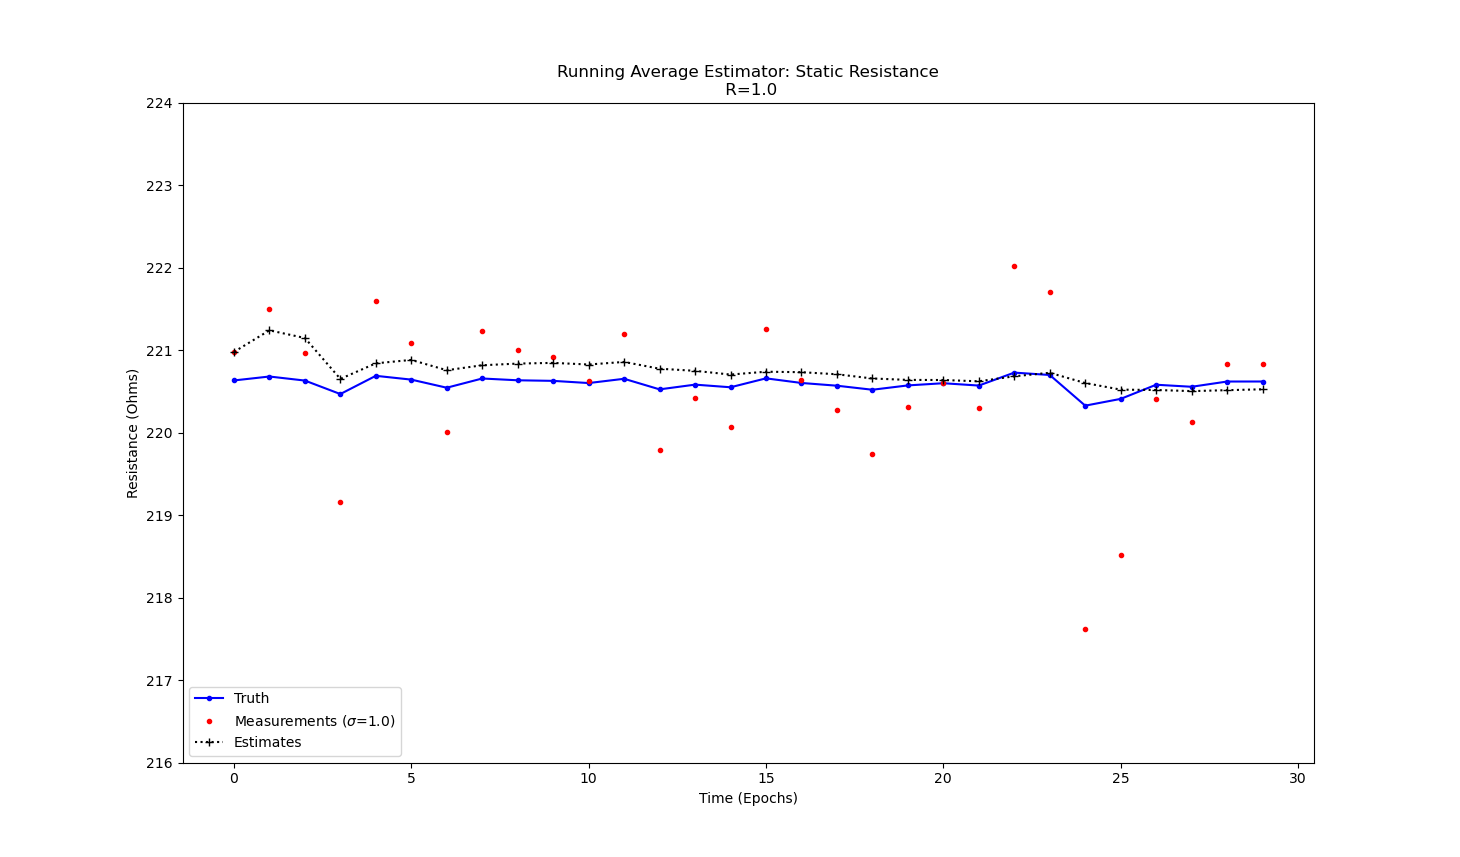
\includegraphics[width=0.95\textwidth]{\dayonesegtwo/run_avg_demo_musicarroll.png}
					\caption{{\tiny Simple Running Average Estimator}}
				\end{subfigure}
				\hfill
				\begin{subfigure}[b]{0.45\textwidth}
					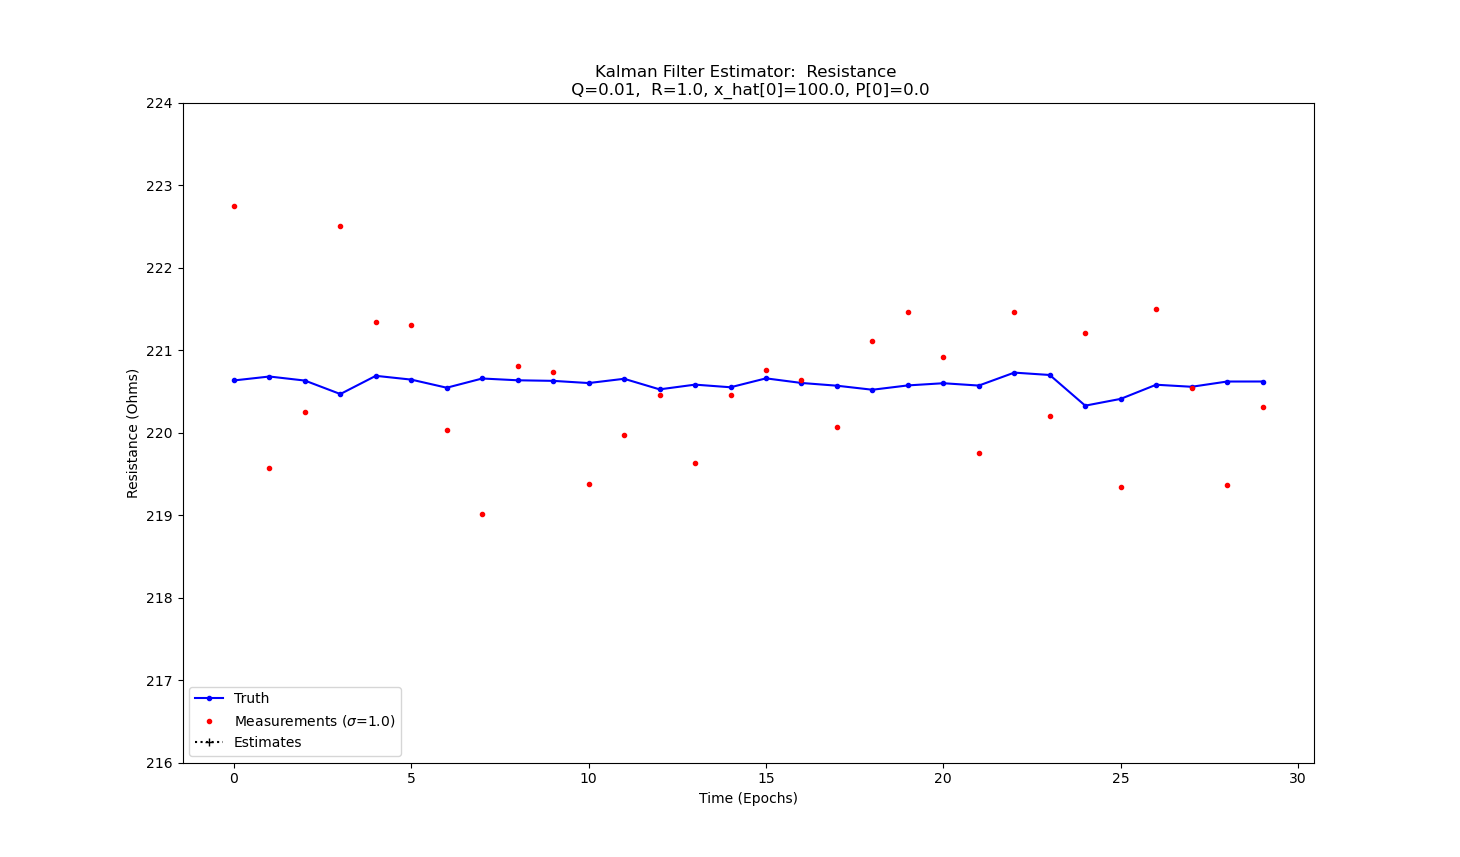
\includegraphics[width=0.95\textwidth]{\dayonesegtwo/kf_resistor_demo_musicarroll.png}
					\caption{{\tiny Kalman Estimator}}
				\end{subfigure}
				\caption{{\small Comparing Running Average and Kalman Estimators \textbf{with process noise!!!}}}
				
			\end{figure}
		}
	\begin{itemize}
		\onslide<3->{\item See run\_avg\_demo\_musicarroll.py in student\_contrib folder on github.}
	\end{itemize}
		
	
	\onslide<4->{\center --------------------------------------------------------------------}
	
\end{frame}


\begin{frame}

  \onslide<1->{\frametitle{Answers to Exercises}
	\framesubtitle{Constant Velocity Motion}
}
\begin{enumerate}
\setcounter{enumi}{4}

  \onslide<2->{\item Calculate the Kalman gain of the non-accelerated motion example.  Hint:  It looks a lot like the 
gain for the damped harmonic oscillator.}
\begin{itemize}

		\onslide<3->{  \item The gain equation $\genkalgaineq$ looks like this:}
\begin{align*}
\onslide<3->{ K &=
	\begin{bmatrix}
	p_{11} & p_{12}\\
	p_{21} & p_{22}
	\end{bmatrix}
	\begin{bmatrix}1\\
	0
	\end{bmatrix}
	\left( \begin{bmatrix}1 & 0\end{bmatrix}\begin{bmatrix}
	p_{11} & p_{12}\\
	p_{21} & p_{22}
	\end{bmatrix}
	\begin{bmatrix}
	1\\ 
	0
	\end{bmatrix}
	+\sigma^2
	\right)^{-1}\\}
\onslide<4->{&=
	\begin{bmatrix}
	\dfrac{p_{11}}{p_{11}+\sigma^2}\\
	\dfrac{p_{21}}{p_{11}+\sigma^2}
	\end{bmatrix},}
\end{align*}
\onslide<5->{where we have once again suppressed the minus(-) superscripts and time step variable $j$ on the right hand side.}

  \onslide<6->{\item This is identical to the gain of the damped harmonic oscillator.  The structure of the $P,R,H$ matrices are the same, so the gain is identical.
}
\end{itemize}

\end{enumerate}
\onslide<7->{\center --------------------------------------------------------------------}
\end{frame}

\begin{frame}
	
	\onslide<1->{\frametitle{Answers to Exercises}
		\framesubtitle{Constant Velocity Motion}
	}
	\begin{enumerate}
		\setcounter{enumi}{5}
		
		\onslide<2->{\item Modify the measurement model in your own copy of  constant\_velocity.py by adding a velocity sensor.  (Be sure to modify both the H and R matrices.)}
\begin{itemize}
		\onslide<3->{
	\item To add a second measurement, the $z(k)$ column vector will now be a true vector with two rows:  $\coltwoveck{z}{k}$.
}

\onslide<4->{
	\item And this means the $H$ matrix and the $R$ matrix have to change.
}

\onslide<5->{
	\item $H=\begin{bmatrix}
	1 & 0\\
	0 & 1
	\end{bmatrix}$ and
	$R=\begin{bmatrix}
	\sigma^2_1\\
	\sigma^2_2
	\end{bmatrix}$\\
	and thus the new measurement model is:
	\begin{equation}
	\coltwoveck{z}{k}= \begin{bmatrix}
	1 & 0\\
	0 & 1
	\end{bmatrix}
	\coltwoveck{x}{k} + \begin{bmatrix}
	v_1\\
	v_2
	\end{bmatrix},
	\end{equation}
	where the $v_i$ are Gaussian, zero-mean, but $v_1$ has variance $\sigma^2_1$ and $v_2$ has variance $\sigma^2_2$.
}
\end{itemize}
		
	\end{enumerate}
	\onslide<6->{\center --------------------------------------------------------------------}
\end{frame}

\begin{frame}
	
	\onslide<1->{\frametitle{Answers to Exercises}
		\framesubtitle{Constant Velocity Motion}
	}
	\begin{enumerate}
		\setcounter{enumi}{6}
		\onslide<2->{\item How do the dimensions of the Kalman gain matrix change after modifying the measurement model in the above manner?}

\begin{itemize}		
		\onslide<3->{\item The number of columns of $K$ must match the number of rows of $z$.
		}
		
		\onslide<4->{\item The number of rows of $K$ must match the number rows in $x$.
		}
		
		\onslide<5->{\item Thus, $K$ will be 2x2.
		}
\end{itemize}
		
	\end{enumerate}
	\onslide<6->{\center --------------------------------------------------------------------}
\end{frame}

\begin{frame}
	
	\onslide<1->{\frametitle{Answers to Exercises}
		\framesubtitle{Constant Velocity Motion}
	}
	\begin{enumerate}
		\setcounter{enumi}{7}
		
		\onslide<2->{\item By how much does the RMS error accuracy of the velocity estimation change with the addition of a direct velocity sensor?}
\begin{itemize}		
	\onslide<3->{\item See the script constant\_velocity\_musicarroll.py in the student\_contrib folder on github, which is a modified version of the original script constant\_velocity.py in the src folder on github.
	}
	
	\onslide<4->{\item Both scripts were run with identical initial values for the key parameters. 
	}
	
	\onslide<5->{\item The performance improvement with the velocity sensor is striking \\ { \footnotesize RMS pos error w/o sensor:  40\% reduction (1.08 vs. 0.668m)\\
		RMS vel error w/o sensor: 60\% reduction (0.2481 vs. 0.0973m/s)}
	}
\end{itemize}
		
	\end{enumerate}
	\onslide<6->{\center --------------------------------------------------------------------}
\end{frame}

\begin{frame}
	
	\onslide<1->{\frametitle{Answers to Exercises}
		\framesubtitle{Constant Velocity Motion: TME Plots w/o Vel Sensor}
	}
	\onslide<2->{
	\begin{figure}
	
	\hfill
		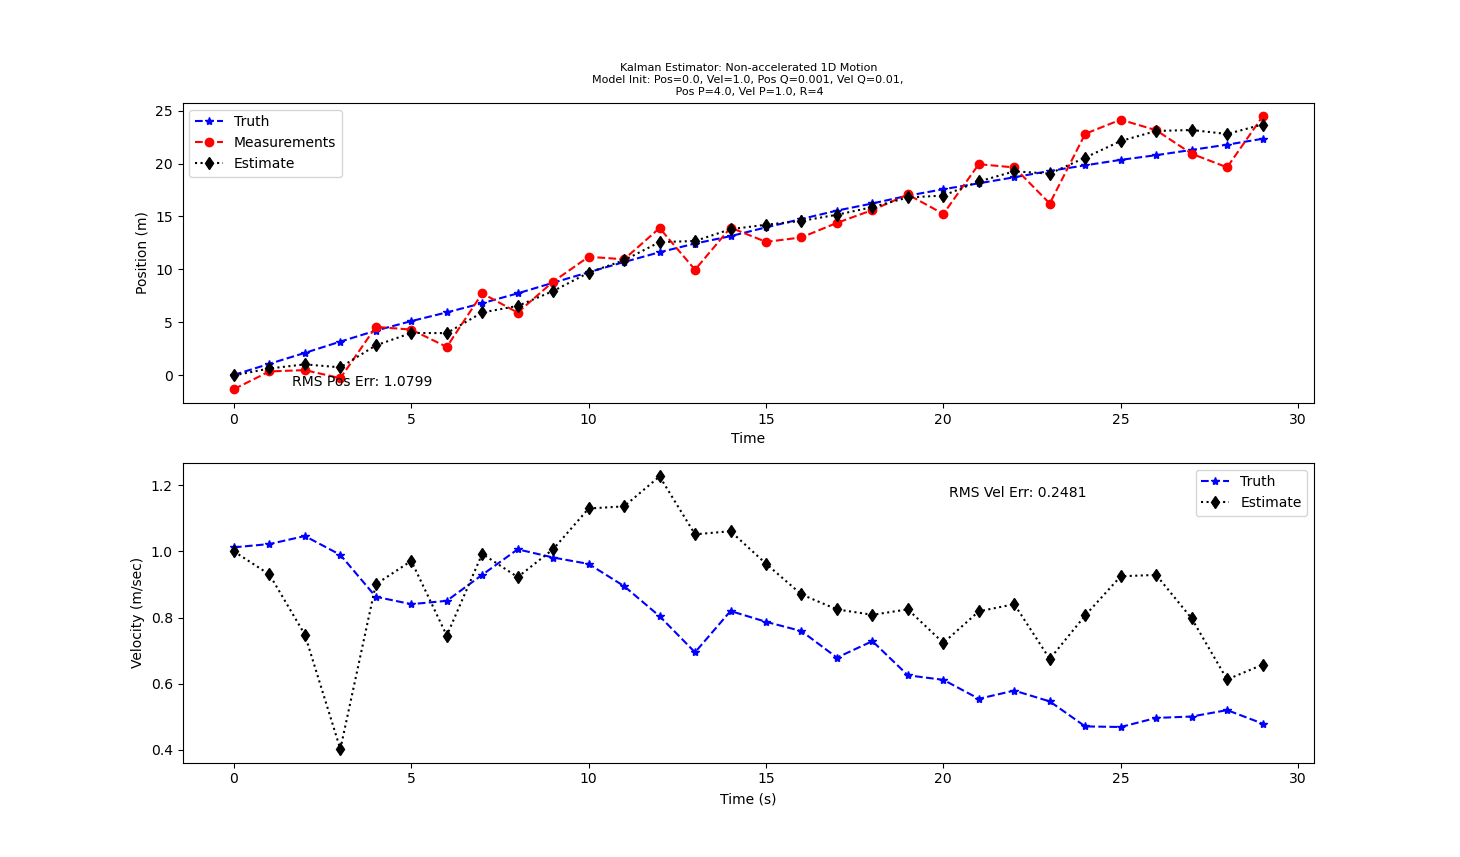
\includegraphics[width=0.95\textwidth]{\dayonesegtwo/const_vel_w_proc_noise_wo_vel_sensor.png}
	\caption{{\small TME Plots Without Velocity Sensor}}
	
\end{figure}
}


	\onslide<3->{\center --------------------------------------------------------------------}
\end{frame}

\begin{frame}
	
	\onslide<1->{\frametitle{Answers to Exercises}
		\framesubtitle{Constant Velocity Motion: TME Plots w/ Vel Sensor}
	}
	\onslide<2->{
		\begin{figure}
			
			\hfill
				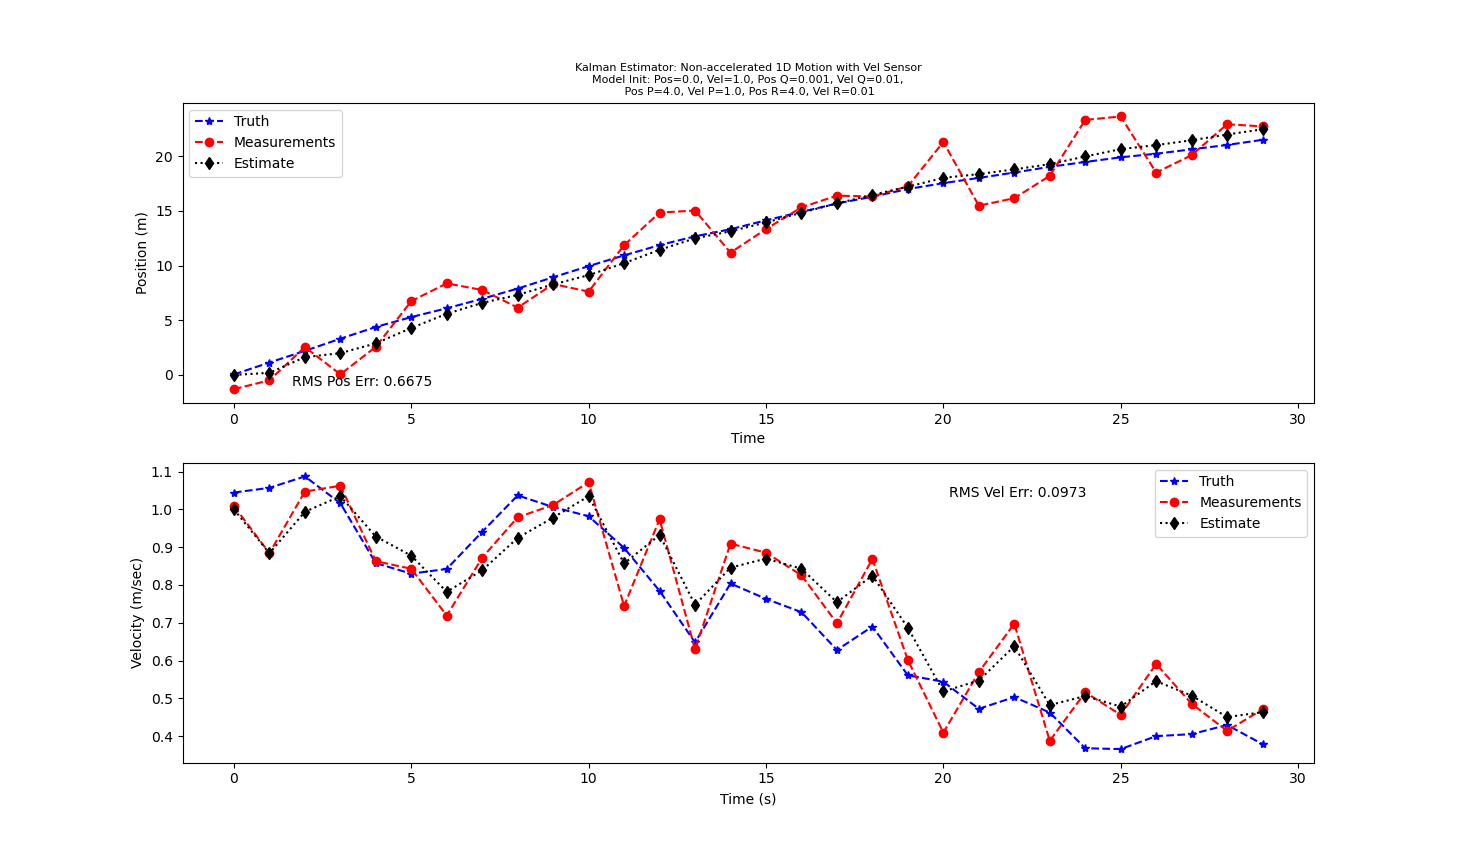
\includegraphics[width=0.95\textwidth]{\dayonesegtwo/const_vel_w_proc_noise_w_vel_sensor.png}
			\caption{{\small TME Plots With Velocity Sensor}}
			
		\end{figure}
	}
	
	
	\onslide<3->{\center --------------------------------------------------------------------}
\end{frame}


\begin{frame}
	
	\onslide<1->{\frametitle{Answers to Exercises}
		\framesubtitle{Constant Velocity Motion: Pos Sawtooth w/o Vel Sensor}
	}
	\onslide<2->{
		\begin{figure}
			
			\hfill
				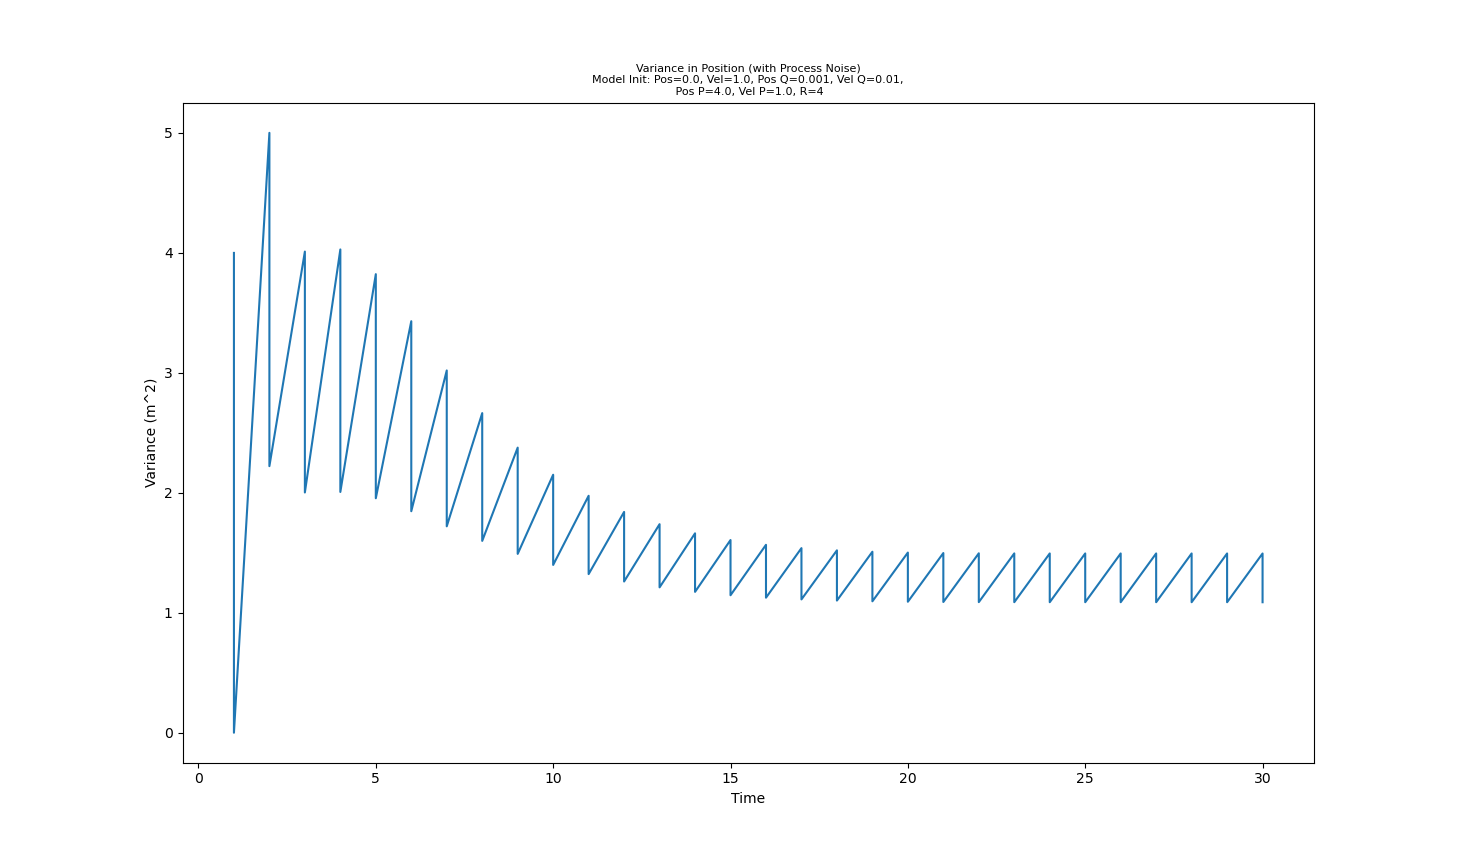
\includegraphics[width=0.95\textwidth]{\dayonesegtwo/const_vel_pos_sawtooth_w_proc_noise_wo_vel_sensor.png}
			\caption{{\small Position Sawtooth \textbf{Without} Velocity Sensor}}
			
		\end{figure}
	}
	
	
	\onslide<3->{\center --------------------------------------------------------------------}
\end{frame}


\begin{frame}
	
	\onslide<1->{\frametitle{Answers to Exercises}
		\framesubtitle{Constant Velocity Motion: Pos Sawtooth w/ Vel Sensor}
	}
	\onslide<2->{
		\begin{figure}
			
			\hfill
				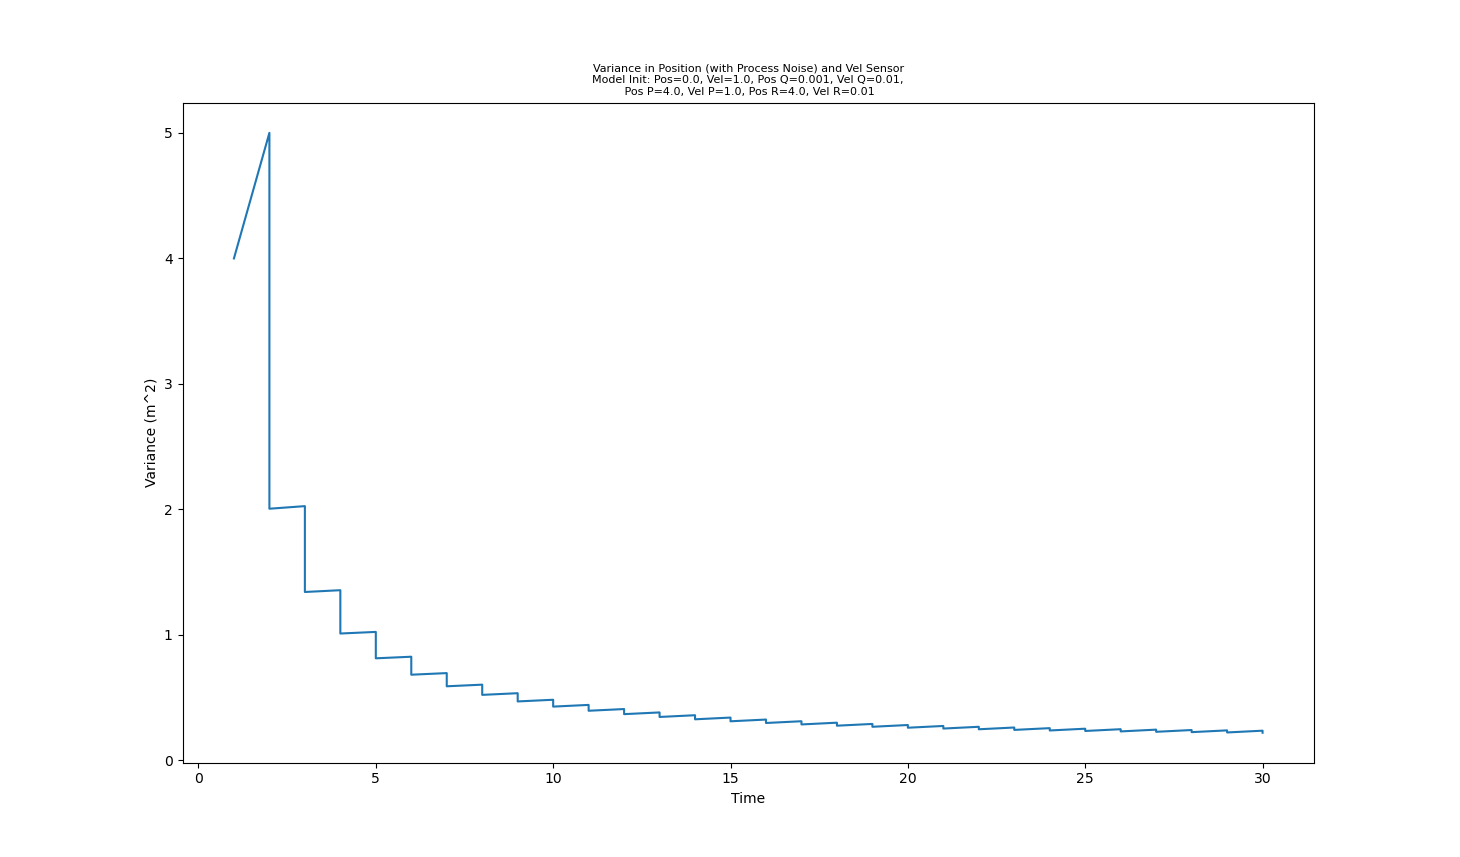
\includegraphics[width=0.95\textwidth]{\dayonesegtwo/const_vel_pos_sawtooth_w_proc_noise_w_vel_sensor.png}
			\caption{{\small Position Sawtooth \textbf{With} Velocity Sensor}}
			
		\end{figure}
	}
	
	
	\onslide<3->{\center --------------------------------------------------------------------}
\end{frame}


\begin{frame}
	
	\onslide<1->{\frametitle{Answers to Exercises}
		\framesubtitle{Constant Velocity Motion: Vel Sawtooth w/o Vel Sensor}
	}
	\onslide<2->{
		\begin{figure}
			
			\hfill
				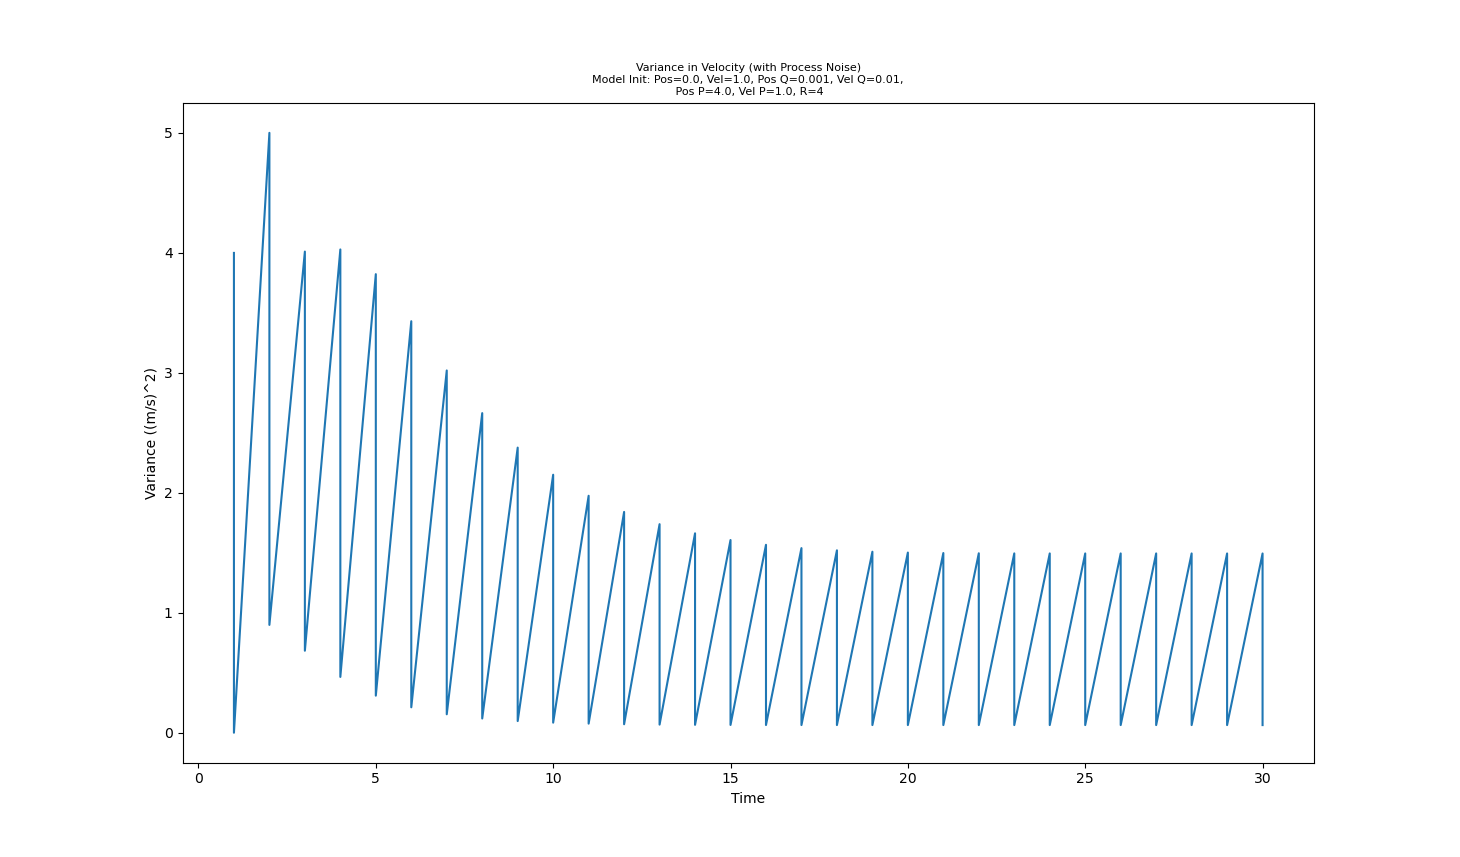
\includegraphics[width=0.95\textwidth]{\dayonesegtwo/const_vel_vel_sawtooth_w_proc_noise_wo_vel_sensor.png}
			\caption{{\small Velocity Sawtooth \textbf{Without} Velocity Sensor}}
			
		\end{figure}
	}
	
	
	\onslide<3->{\center --------------------------------------------------------------------}
\end{frame}


\begin{frame}
	
	\onslide<1->{\frametitle{Answers to Exercises}
		\framesubtitle{Constant Velocity Motion: Vel Sawtooth w/ Vel Sensor}
	}
	\onslide<2->{
		\begin{figure}
			
			\hfill
				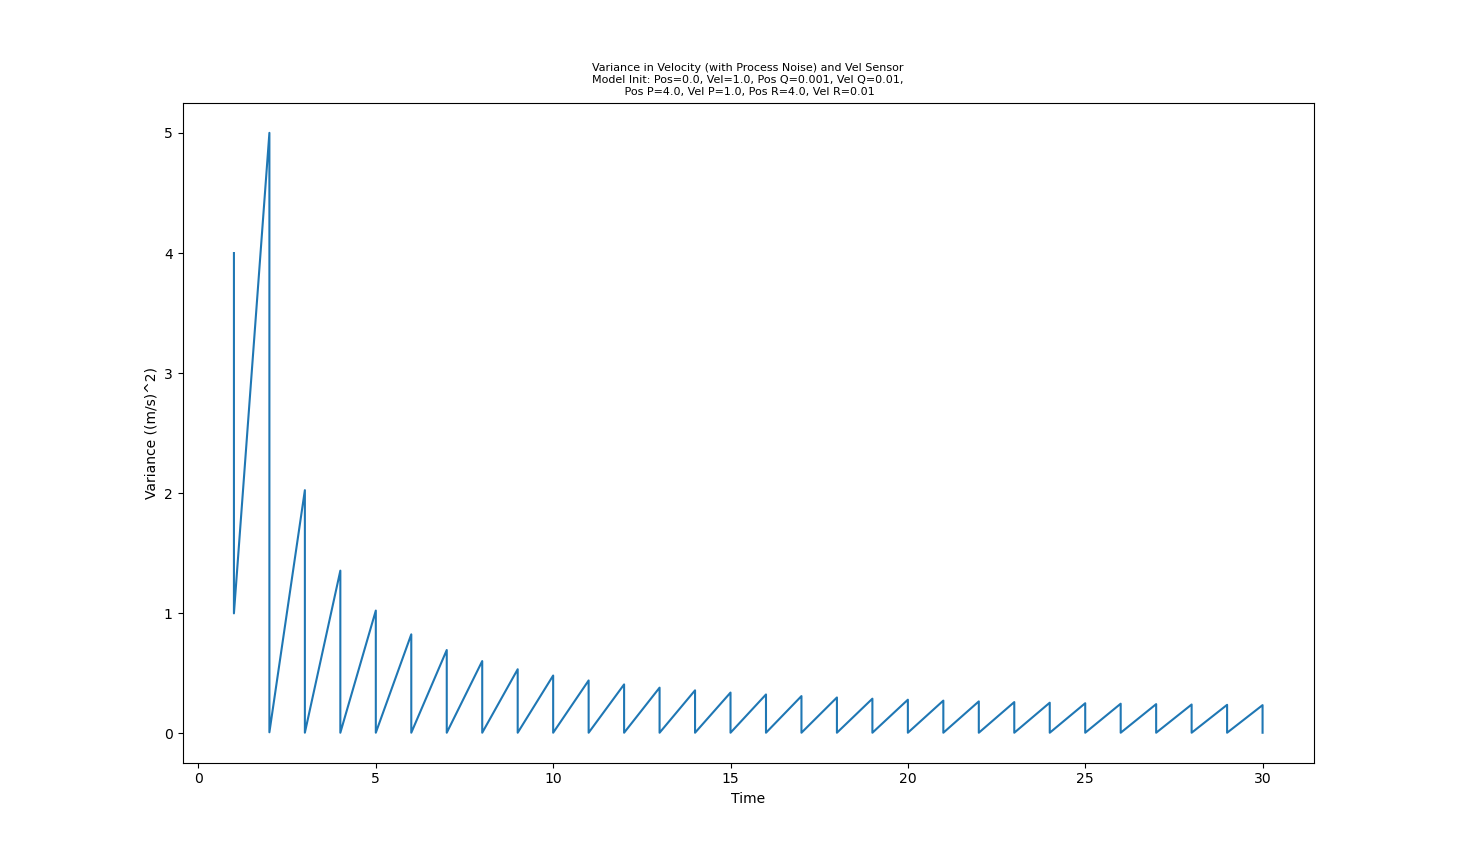
\includegraphics[width=0.95\textwidth]{\dayonesegtwo/const_vel_vel_sawtooth_w_proc_noise_w_vel_sensor.png}

			\caption{{\small Velocity Sawtooth \textbf{With} Velocity Sensor}}
			
		\end{figure}
	}
	
	
	\onslide<3->{\center --------------------------------------------------------------------}
\end{frame}


\begin{frame}
	
	\onslide<1->{\frametitle{Answers to Exercises}
		\framesubtitle{Damped Harmonic Oscillator}
	}
	\begin{enumerate}
		\setcounter{enumi}{8}		
		
		\onslide<2->{\item Modify the measurement model for the damped harmonic oscillator in your own copy of damposc.py by adding a direct velocity sensor.}
		\begin{itemize}
		\onslide<3->{\item Same mods as those made to the constant velocity model. $\Phi$ doesn't change.}

\onslide<4->{\item Changes to $z,H, R$ }

\onslide<5->{\item See damposc\_musicarroll.py on github in student\_contrib subfolder.
}
		\end{itemize}
	\end{enumerate}
	\onslide<6->{\center --------------------------------------------------------------------}
\end{frame}

\begin{frame}
	
	\onslide<1->{\frametitle{Answers to Exercises}
		\framesubtitle{Damped Harmonic Oscillator}
	}
	\begin{enumerate}
		\setcounter{enumi}{9}		
		
		\onslide<2->{\item By how much does the RMS error accuracy of the velocity estimation change with the addition of a direct velocity sensor?}
		\begin{itemize}
		\onslide<3->{\item Pos Error \textbf{increase}: 18\% }

\onslide<4->{\item Vel Error \textbf{decrease}: 52\% }

\onslide<5->{\item Pos Error should have decreased.  That it didn't is probably due either to inconsistency of initial values and/or large transients overwhelming the RMS averaging.  Please comment on what you think the cause is!
}
		\end{itemize}
	\end{enumerate}
	\onslide<6->{\center --------------------------------------------------------------------}
\end{frame}

\begin{frame}
	
	\onslide<1->{\frametitle{Answers to Exercises}
		\framesubtitle{Damped Harmonic Oscillator: TME Plot w/o Vel Sensor}
	}
	\onslide<2->{
		\begin{figure}
			
			\hfill
			\includegraphics[width=0.95\textwidth]{\dayonesegtwo/damposc_tme_wo_vel_sensor.png}
			
			\caption{{\small TME Plot w/o Vel Sensor}}
			
		\end{figure}
	}
	
	
	\onslide<3->{\center --------------------------------------------------------------------}
\end{frame}

\begin{frame}
	
	\onslide<1->{\frametitle{Answers to Exercises}
		\framesubtitle{Damped Harmonic Oscillator: TME Plot w/ Pos and Vel Sensors}
	}
	\onslide<2->{
		\begin{figure}
			
			\hfill
			\includegraphics[width=0.95\textwidth]{\dayonesegtwo/damposc_tme_w_vel_sensor.png}
			
			\caption{{\small TME Plot w/ Pos and Vel Sensors}}
			
		\end{figure}
	}
	
	
	\onslide<3->{\center --------------------------------------------------------------------}
\end{frame}

\begin{frame}
	
	\onslide<1->{\frametitle{Answers to Exercises}
		\framesubtitle{Damped Harmonic Oscillator: Position Variance Sawtooth w/o Vel Sensor}
	}
	\onslide<2->{
		\begin{figure}
			
			\hfill
			\includegraphics[width=0.95\textwidth]{\dayonesegtwo/damposc_sawtooth_pos_w_vel_sensor.png}
			
			\caption{{\small Position Variance Sawtooth w/o Vel Sensor}}
			
		\end{figure}
	}
	
	
	\onslide<3->{\center --------------------------------------------------------------------}
\end{frame}

\begin{frame}
	
	\onslide<1->{\frametitle{Answers to Exercises}
		\framesubtitle{Damped Harmonic Oscillator: Position Variance Sawtooth w/ Vel Sensor}
	}
	\onslide<2->{
		\begin{figure}
			
			\hfill
			\includegraphics[width=0.95\textwidth]{\dayonesegtwo/damposc_sawtooth_pos_w_vel_sensor.png}
			
			\caption{{\small Position Variance Sawtooth w/ Vel Sensor}}
			
		\end{figure}
	}
	
	
	\onslide<3->{\center --------------------------------------------------------------------}
\end{frame}



\begin{frame}
	
	\onslide<1->{\frametitle{Answers to Exercises}
		\framesubtitle{Damped Harmonic Oscillator: Velocity Variance Sawtooth w/o Vel Sensor}
	}
	\onslide<2->{
		\begin{figure}
			
			\hfill
			\includegraphics[width=0.95\textwidth]{\dayonesegtwo/damposc_sawtooth_vel_wo_vel_sensor.png}
			
			\caption{{\small Velocity Variance Sawtooth w/o Vel Sensor}}
			
		\end{figure}
	}
	
	
	\onslide<3->{\center --------------------------------------------------------------------}
\end{frame}

\begin{frame}
	
	\onslide<1->{\frametitle{Answers to Exercises}
		\framesubtitle{Damped Harmonic Oscillator: Velocity Variance Sawtooth w/ Vel Sensor}
	}
	\onslide<2->{
		\begin{figure}
			\hfill
			\includegraphics[width=0.95\textwidth]{\dayonesegtwo/damposc_sawtooth_vel_w_vel_sensor.png}
			
			\caption{{\small Velocity Variance Sawtooth w/ Vel Sensor}}
			
		\end{figure}
	}
	
	
	\onslide<3->{\center --------------------------------------------------------------------}
\end{frame}



\begin{frame}
	
	\onslide<1->{\frametitle{Answers to Exercises}
		\framesubtitle{Damped Harmonic Oscillator}
	}
	\begin{enumerate}
		\setcounter{enumi}{10}		
		
		\onslide<2->{\item Add a second sawtooth plot for the velocity state estimation uncertainty.   How do the sawtooth patterns change with each of the mods above?}
	\begin{itemize}
		\onslide<3->{\item See previous slides.}

\onslide<4->{\item Sawtooth patterns show marked improvement in velocity variance  }

\onslide<5->{\item But position variance did not improve.  It depends on the accuracy of the velocity sensor.}
	\end{itemize}	
	
	\end{enumerate}
	\onslide<6->{\center --------------------------------------------------------------------}
\end{frame}



\begin{frame}
  \onslide<1->{
	\frametitle{Summary} 
	\framesubtitle{Vector Check}
  }

\begin{itemize}
  \onslide<2->{
\item Where are we?  
}

\begin{itemize}

\onslide<3->{\item Presented answers to 11 exercises }
\onslide<4->{\item 
	Reminder: Original python scripts are in {\small \url{https://github.com/musicarroll/kalman_course/src}}and modified python scripts (and some plots) are located in {\small \url{https://github.com/musicarroll/kalman_course/student_contrib}}
} 

\end{itemize}

\onslide<6->{
\item What's next?  
}
\begin{itemize}
  \onslide<7->{ \item In the next video, we will start a new playlist on State Space Concepts }
\end{itemize}

\end{itemize}
\onslide<8->{\center --------------------------------------------------------------------}
\end{frame}


\end{document}
